\documentclass[aspectratio=169]{beamer}

\usepackage{color}
\definecolor{airforceblue}{rgb}{0.36, 0.54, 0.66}
\definecolor{blue-green}{rgb}{0.0, 0.87, 0.87}
\definecolor{blue-violet}{rgb}{0.54, 0.17, 0.89}
\definecolor{cadet}{rgb}{0.33, 0.41, 0.47}
\definecolor{cordovan}{rgb}{0.54, 0.25, 0.27}

\mode<presentation>
{
    \usetheme{Madrid}
    \usefonttheme{professionalfonts} 
	\setbeamercolor{local structure}{fg=blue-green}
    \setbeamertemplate{itemize subitem}{\color{cordovan}$\blacktriangleright$}
}


\usepackage[utf8]{inputenc}
\usetheme{Madrid}
\usecolortheme{beaver}

\title{Comunicação em Datacenters}
\subtitle{Gerência de Redes}
\author[Leandro Silva, Luís Felipe] % (optional, for multiple authors)
{Leandro Souza da  Silva \\ Luís Felipe Mattos}
\institute{IC - Unicamp}


\date{ 06 de Dezembro de 2016 }
\logo{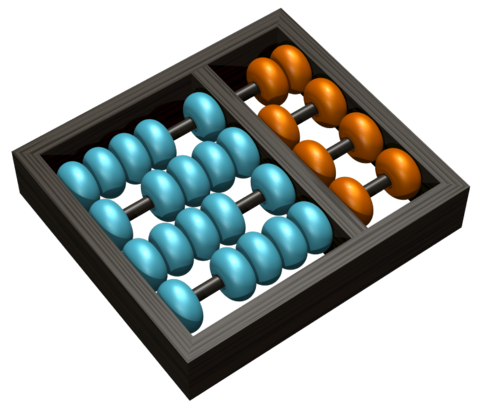
\includegraphics[height=1.0cm]{logo.png}}
 
\AtBeginSection[]
{
  \begin{frame}<beamer>{Sumário}
    \tableofcontents[currentsection, currentsubsection]
  \end{frame}
}


\begin{document}

\frame{\titlepage}

\section{Introdução}
	\begin{frame} {Introdução}
	
		
	 \begin{itemize}
	 \setlength\itemsep{2em}
	 	\Large
	 	\item
	 		Com o crescimento da computação em nuvem, os datacenters passaram a receber funções novas.
	 		
	 \item
	  	Certas aplicações necessitam de certos requisitos:
	  	\begin{itemize}
	 		\item
	 			Escalabilidade
	 	
			\item
			 	Tolerância a Falhas
			\item
			 	Latêcia
			 	
			 \item
			 	Capacidade da Rede
			 \item
			 	Virtualização	 			
	 	\end{itemize}
	 		 	
	 \end{itemize}
		
	\end{frame}



\section{Motivação} 

	\begin{frame} {Motivação}
			
			\centering
			\Large
				 O consumo de dados pelos usuários está crescendo exponencialmente a cada ano.
				\begin{figure}[ht]    
				    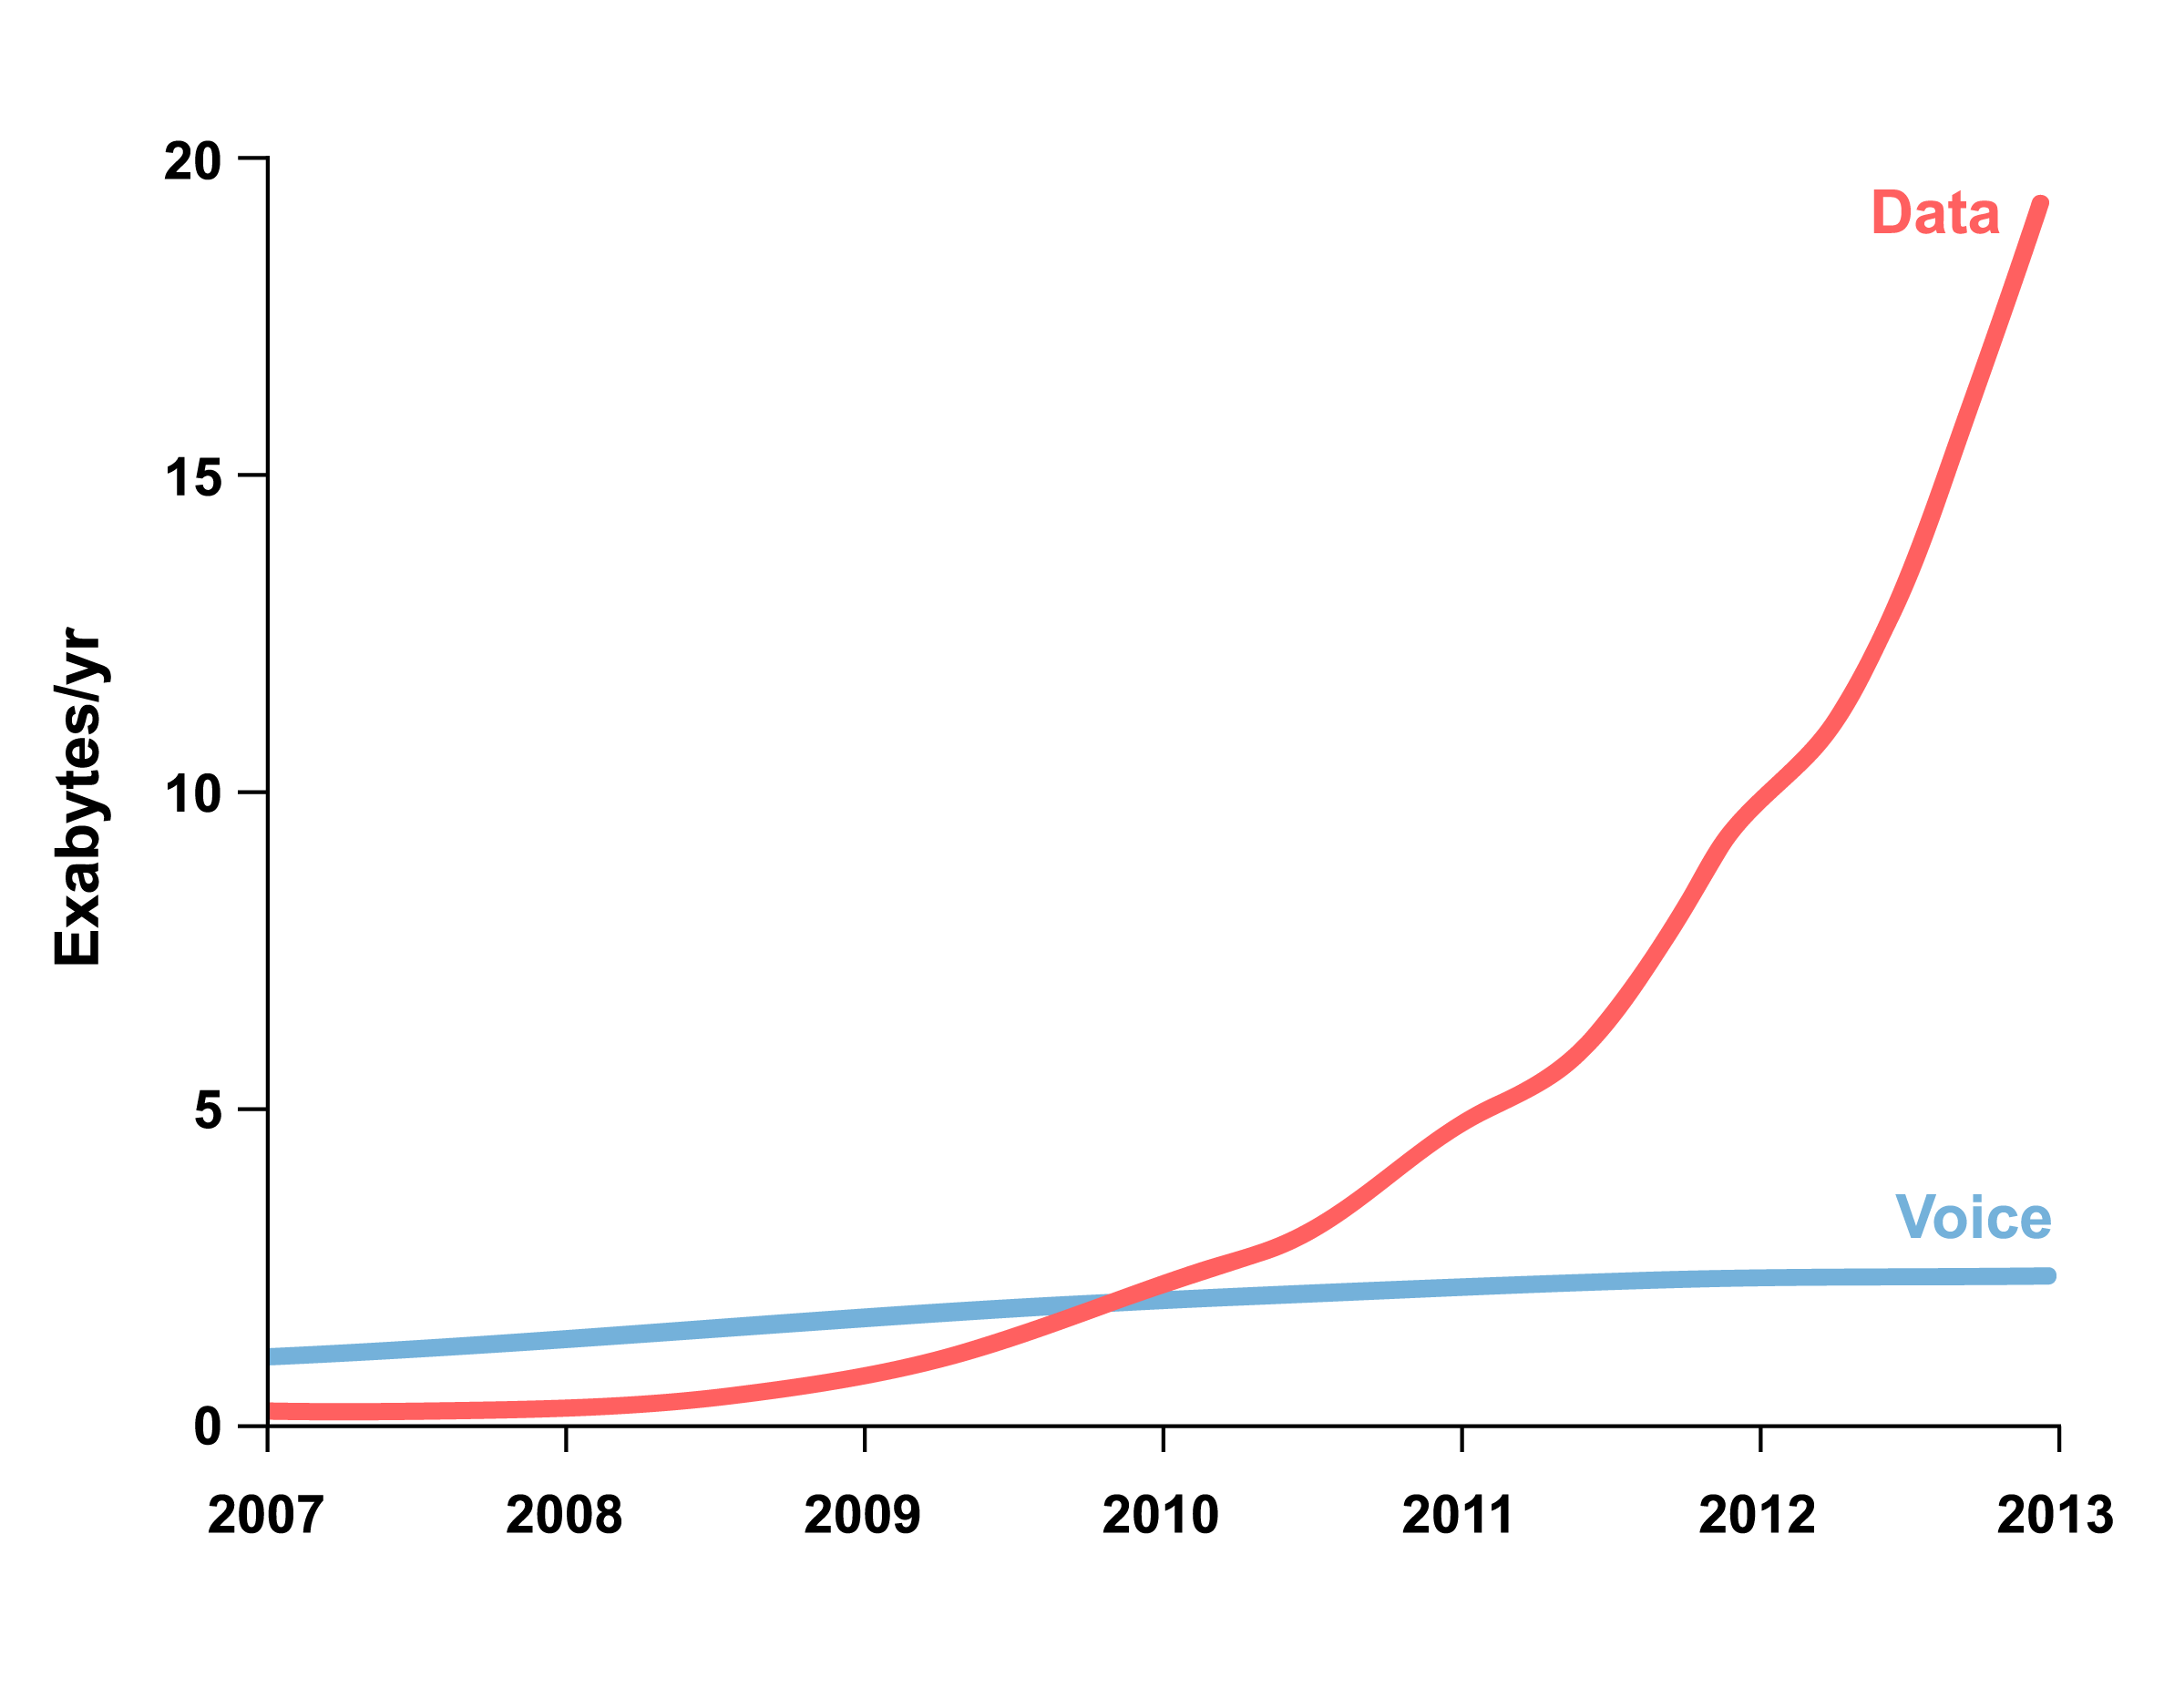
\includegraphics[scale=0.3]{consumo.png}
				    \caption{Consumo de dados e voz}
				    \label{fig:sample_figure}
				\end{figure}

	\end{frame}
	
		\begin{frame} {Motivação}
			
			\centering
			\normalsize	 
				Por causa disso, o número de servidores em Data Centers deve crescer exponencialmente para acompanhar a demanda, o que traz dificuldades em desenvolver redes eficientes e de baixo custo.
			\begin{figure}[ht]
	   
			   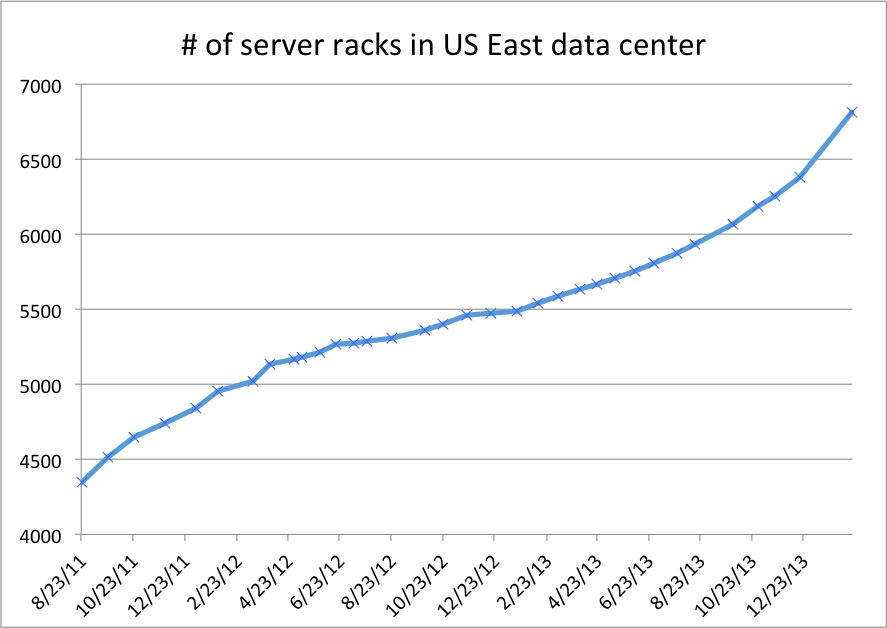
\includegraphics[scale=0.45]{servidores.png}
			    \caption{Número de servidores racks}
			    \label{fig:sample_figure}
			\end{figure}
		
		\end{frame}
		
		\begin{frame} {Motivação}
				
			\Large
			Disponibilidade de dados e segurança se tornaram aplicações críticas.
			
		\end{frame}
				
			
		\begin{frame} {Motivação}
				
			\Large
			Por outro lado, a criação de novas tecnologias faz com que o custo dos componentes seja cada vez menor.
			\begin{figure}[ht]    
						    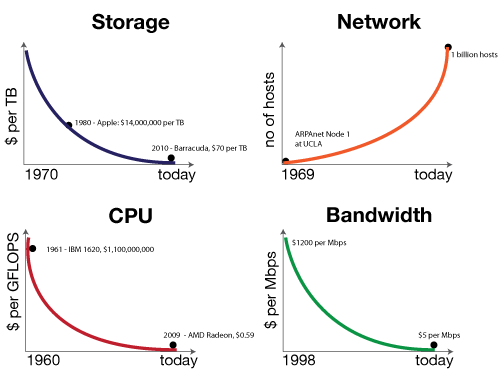
\includegraphics[scale=0.35]{custo.png}
						    \caption{Custo de tecnologias}
						    \label{fig:sample_figure}
						\end{figure}
		\end{frame}	
			
		
	
\section{Topologias} {Toplogias}
	\subsection{Tradicionais}
	\subsection{SDN}
		
	\begin{frame} 
		Ponha aqui seu texto
	\end{frame}	

\section{Protocolos}{Protocolos}
	\subsection{Roteamento}
	\subsection{Comunicação}
			
	\begin{frame} 
		Ponha aqui seu texto
	\end{frame}

\section{Tendências}
	\begin{frame} 
		Ponha aqui seu texto
	\end{frame}

\section{Conclusão}
	\begin{frame} 
		Ponha aqui seu texto
	\end{frame}
		
\section{Pergunta}
	\begin{frame} 
		Ponha aqui seu texto
	\end{frame}
	
\end{document}
